\documentclass[9pt]{article}

\usepackage{amssymb}
\usepackage{amsmath}
\usepackage{amsfonts}
\usepackage{comment}
\usepackage{fancyhdr}
\usepackage{mathrsfs}
\usepackage{enumitem}
\usepackage{graphicx}

\usepackage{tikz}

\voffset = -50pt
%\textheight = 700pt
\addtolength{\textwidth}{60pt}
\addtolength{\evensidemargin}{-30pt}
\addtolength{\oddsidemargin}{-30pt}
%\setlength{\headheight}{44pt}

\newcommand{\qed}{\hfill \ensuremath{\Box}}


\newcommand*\circled[1]{\tikz[baseline=(char.base)]{
            \node[shape=circle,draw,inner sep=2pt] (char) {#1};}}

\newcommand{\Z}{\mathbb{Z}}
\newcommand{\I}{\mathbb{I}}
\newcommand{\M}{\mathbb{M}}
\newcommand{\R}{\mathbb{R}}
\newcommand{\C}{\mathbb{C}}
%\setcounter{section}{-1}

\begin{document}
\topskip0pt
\vspace*{\fill}
\begin{center}
{\Huge \begin{tabular}{@{}ll@{}}
   Class: & CECS 201, Section 7 \\ \\ \\
   Lab: & 9 \\ \\ \\
   Title: & Decade Ripple Counter \\ \\ \\
   Student Name: & Barry Joseph Okonoboh \\ \\ \\
   Due Date: & 11:59:59 P.M., 15, April 2015 \\ \\ \\
   Instructor: & Dan Cregg
\end{tabular}}
\end{center}
\vspace*{\fill}
\newpage
\begin{enumerate}
%%%%%%%%%%%%%%%%%%%%%%%%%%%%%%%%%%%%%%%%01%%%%%%%%%%%%%%%%%%%%%%%%%%%%%%%%%%%%%%
   \item[\textbf{Introduction.}]  In this lab we use T Flip-Flops to create a
   counter that counts modulo ten. That is, a counter that starts from 0, then
   increments on each clock edge by 1, and resets back to 0 upon reaching 10.
   \item[\textbf{Project Description.}] Since we want the counter to reset at the
   decimal number 10, our output will require 4 bits; thus we shall connect four
   T Flip-Flops in sequence, wherein the inverted output of a T Flip-Flop is
   connected to the clock input of the Flip-Flop to its right. Label the Flip-Flops, from left to
   right, $A$, $B$, $C$, and $D$.  The output of $A$ represents the low bit of
   the counter, and the output of $B$ represents the next bit, and so on. The T
   inputs of all Flip-Flops shall be high. Notice that the $A$ toggles its value
   on every clock edge, $B$ on every 2 clock edges, $C$ on every 4 clock edges,
   and $D$ on every 8 clock edges. Since we want the counter to reset at the
   binary value 1010, we shall clear the Flip-Flops by using inverters (on the
   outputs of $A$ and $C$) and a 4-nand gate. 
  	\item[\textbf{Schematic.}] \text{ }
   
             \begin{center}
                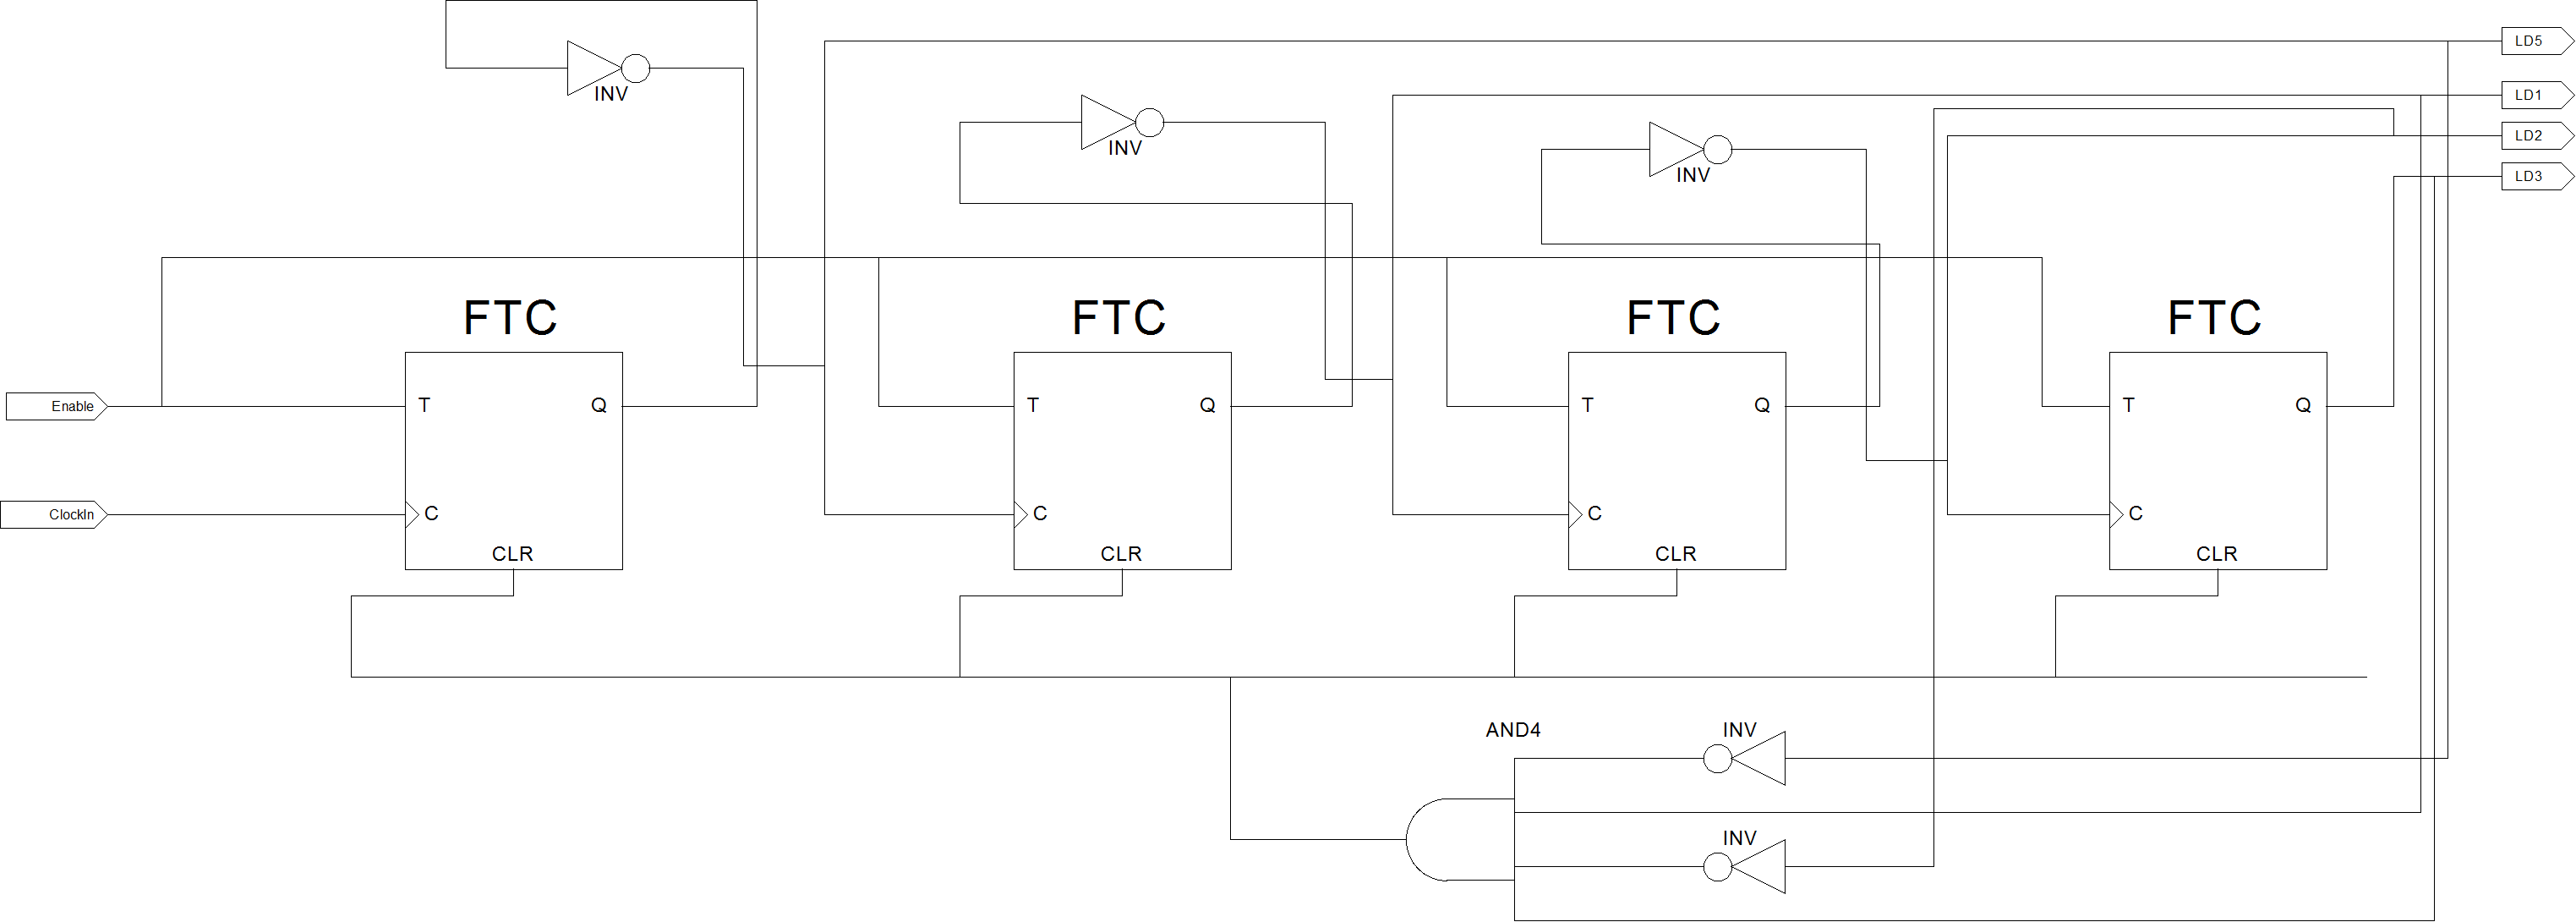
\includegraphics[width=\textwidth]{schematic.png}
             \end{center} 
   
   
\end{enumerate}
\end{document}
